\documentclass[14pt]{extbook}
\usepackage{multicol, enumerate, enumitem, hyperref, color, soul, setspace, parskip, fancyhdr} %General Packages
\usepackage{amssymb, amsthm, amsmath, latexsym, units, mathtools} %Math Packages
\everymath{\displaystyle} %All math in Display Style
% Packages with additional options
\usepackage[headsep=0.5cm,headheight=12pt, left=1 in,right= 1 in,top= 1 in,bottom= 1 in]{geometry}
\usepackage[usenames,dvipsnames]{xcolor}
\usepackage{dashrule}  % Package to use the command below to create lines between items
\newcommand{\litem}[1]{\item#1\hspace*{-1cm}\rule{\textwidth}{0.4pt}}
\pagestyle{fancy}
\lhead{Module4}
\chead{}
\rhead{Version C}
\lfoot{2958-5637}
\cfoot{}
\rfoot{test}
\begin{document}

\begin{enumerate}
\litem{
Graph the equation below.\[ f(x) = -(x-1)^2 + 12 \]\begin{enumerate}[label=\Alph*.]
\begin{multicols}{2}\item 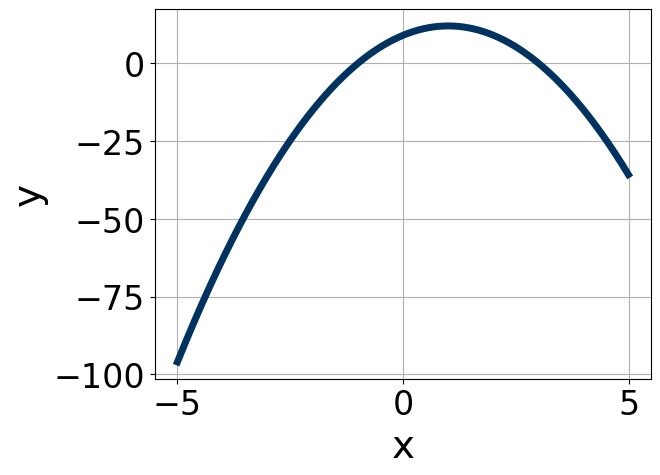
\includegraphics[width = 0.3\textwidth]{../Figures/quadraticEquationToGraphCopyAC.png}\item 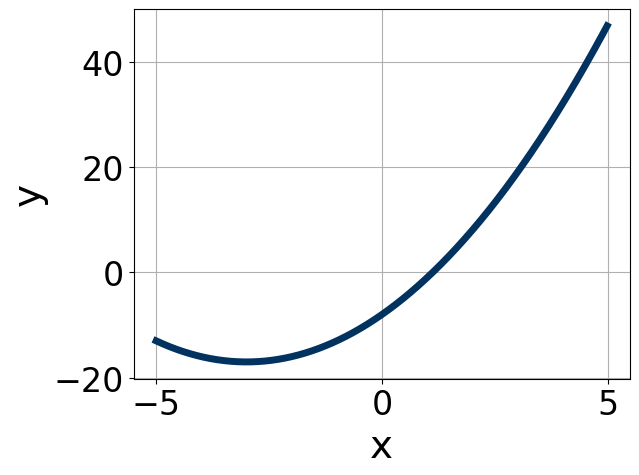
\includegraphics[width = 0.3\textwidth]{../Figures/quadraticEquationToGraphCopyBC.png}\item 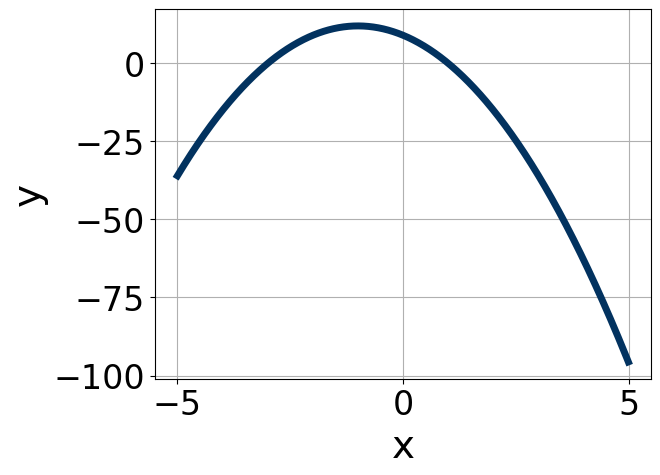
\includegraphics[width = 0.3\textwidth]{../Figures/quadraticEquationToGraphCopyCC.png}\item 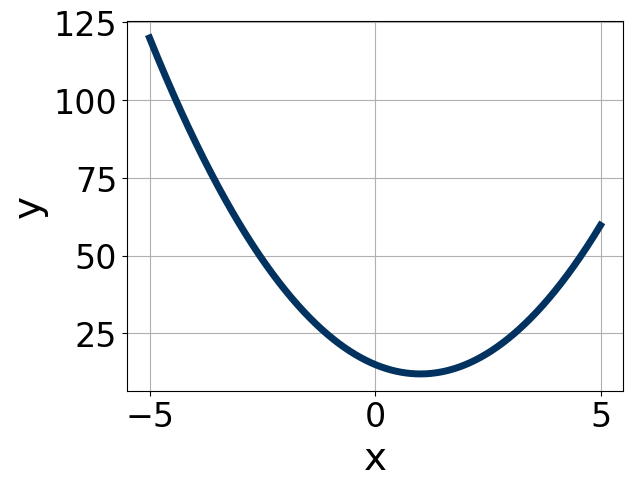
\includegraphics[width = 0.3\textwidth]{../Figures/quadraticEquationToGraphCopyDC.png}\end{multicols}\item None of the above.
\end{enumerate} }
\litem{
Factor the quadratic below. Then, choose the intervals that contain the constants in the form $(ax+b)(cx+d); b \leq d.$\[ 16x^{2} -8 x -15 \]\begin{enumerate}[label=\Alph*.]
\item \( a \in [1.45, 3.08], \hspace*{5mm} b \in [-13, 2], \hspace*{5mm} c \in [7.34, 8.03], \text{ and } \hspace*{5mm} d \in [2, 7] \)
\item \( a \in [7.54, 8.63], \hspace*{5mm} b \in [-13, 2], \hspace*{5mm} c \in [1.34, 2.96], \text{ and } \hspace*{5mm} d \in [2, 7] \)
\item \( a \in [3.05, 5.42], \hspace*{5mm} b \in [-13, 2], \hspace*{5mm} c \in [3.24, 5.71], \text{ and } \hspace*{5mm} d \in [2, 7] \)
\item \( a \in [-0.4, 1.13], \hspace*{5mm} b \in [-21, -17], \hspace*{5mm} c \in [0.39, 1.71], \text{ and } \hspace*{5mm} d \in [12, 13] \)
\item \( \text{None of the above.} \)

\end{enumerate} }
\litem{
Solve the quadratic equation below. Then, choose the intervals that the solutions belong to, with $x_1 \leq x_2$ (if they exist).\[ 20x^{2} -12 x -4 = 0 \]\begin{enumerate}[label=\Alph*.]
\item \( x_1 \in [-5.45, -4.16] \text{ and } x_2 \in [15.6, 17.37] \)
\item \( x_1 \in [-0.35, -0.2] \text{ and } x_2 \in [0.46, 1.49] \)
\item \( x_1 \in [-21.47, -20.53] \text{ and } x_2 \in [21.59, 22.51] \)
\item \( x_1 \in [-0.96, -0.42] \text{ and } x_2 \in [-0.12, 0.64] \)
\item \( \text{There are no Real solutions.} \)

\end{enumerate} }
\litem{
Write the equation of the graph presented below in the form $f(x)=ax^2+bx+c$, assuming  $a=1$ or $a=-1$. Then, choose the intervals that $a, b,$ and $c$ belong to.
\begin{center}
    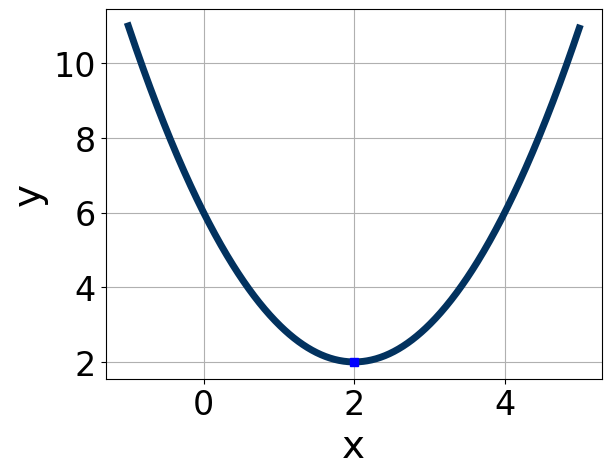
\includegraphics[width=0.5\textwidth]{../Figures/quadraticGraphToEquationC.png}
\end{center}
\begin{enumerate}[label=\Alph*.]
\item \( a \in [0, 7], \hspace*{5mm} b \in [3, 7], \text{ and } \hspace*{5mm} c \in [5, 8] \)
\item \( a \in [0, 7], \hspace*{5mm} b \in [-5, -3], \text{ and } \hspace*{5mm} c \in [5, 8] \)
\item \( a \in [-2, 0], \hspace*{5mm} b \in [3, 7], \text{ and } \hspace*{5mm} c \in [-4, 1] \)
\item \( a \in [0, 7], \hspace*{5mm} b \in [3, 7], \text{ and } \hspace*{5mm} c \in [2, 5] \)
\item \( a \in [-2, 0], \hspace*{5mm} b \in [-5, -3], \text{ and } \hspace*{5mm} c \in [-4, 1] \)

\end{enumerate} }
\litem{
Solve the quadratic equation below. Then, choose the intervals that the solutions belong to, with $x_1 \leq x_2$ (if they exist).\[ 10x^{2} -8 x -5 = 0 \]\begin{enumerate}[label=\Alph*.]
\item \( x_1 \in [-1.58, -1.14] \text{ and } x_2 \in [-0.72, 0.83] \)
\item \( x_1 \in [-0.9, 0.34] \text{ and } x_2 \in [0.49, 1.82] \)
\item \( x_1 \in [-16.09, -14.96] \text{ and } x_2 \in [16.12, 17.01] \)
\item \( x_1 \in [-4.15, -3.76] \text{ and } x_2 \in [11.97, 12.52] \)
\item \( \text{There are no Real solutions.} \)

\end{enumerate} }
\litem{
Solve the quadratic equation below. Then, choose the intervals that the solutions $x_1$ and $x_2$ belong to, with $x_1 \leq x_2$.\[ 15x^{2} -2 x -24 = 0 \]\begin{enumerate}[label=\Alph*.]
\item \( x_1 \in [-3.65, -3.59] \text{ and } x_2 \in [0.41, 0.55] \)
\item \( x_1 \in [-0.68, -0.3] \text{ and } x_2 \in [2.35, 2.74] \)
\item \( x_1 \in [-18.38, -17.52] \text{ and } x_2 \in [19.64, 20.09] \)
\item \( x_1 \in [-1.25, -0.62] \text{ and } x_2 \in [1.32, 1.36] \)
\item \( x_1 \in [-6.04, -5.76] \text{ and } x_2 \in [0.24, 0.37] \)

\end{enumerate} }
\litem{
Solve the quadratic equation below. Then, choose the intervals that the solutions $x_1$ and $x_2$ belong to, with $x_1 \leq x_2$.\[ 10x^{2} -33 x -54 = 0 \]\begin{enumerate}[label=\Alph*.]
\item \( x_1 \in [-3, -0.8] \text{ and } x_2 \in [4.29, 5.8] \)
\item \( x_1 \in [-0.9, 1.2] \text{ and } x_2 \in [12.38, 14.74] \)
\item \( x_1 \in [-4.1, -1.9] \text{ and } x_2 \in [1.13, 2.94] \)
\item \( x_1 \in [-6.7, -5.1] \text{ and } x_2 \in [-0.59, 1.02] \)
\item \( x_1 \in [-13.5, -11.5] \text{ and } x_2 \in [43.59, 46.44] \)

\end{enumerate} }
\litem{
Factor the quadratic below. Then, choose the intervals that contain the constants in the form $(ax+b)(cx+d); b \leq d.$\[ 81x^{2} +54 x + 8 \]\begin{enumerate}[label=\Alph*.]
\item \( a \in [1, 2], \hspace*{5mm} b \in [18, 24], \hspace*{5mm} c \in [0.5, 1.9], \text{ and } \hspace*{5mm} d \in [34, 38] \)
\item \( a \in [3, 4], \hspace*{5mm} b \in [-5, 8], \hspace*{5mm} c \in [25.8, 30.8], \text{ and } \hspace*{5mm} d \in [-2, 6] \)
\item \( a \in [21, 29], \hspace*{5mm} b \in [-5, 8], \hspace*{5mm} c \in [2.6, 3.1], \text{ and } \hspace*{5mm} d \in [-2, 6] \)
\item \( a \in [9, 12], \hspace*{5mm} b \in [-5, 8], \hspace*{5mm} c \in [8.1, 11.5], \text{ and } \hspace*{5mm} d \in [-2, 6] \)
\item \( \text{None of the above.} \)

\end{enumerate} }
\litem{
Graph the equation below.\[ f(x) = -(x+3)^2 + 12 \]\begin{enumerate}[label=\Alph*.]
\begin{multicols}{2}\item 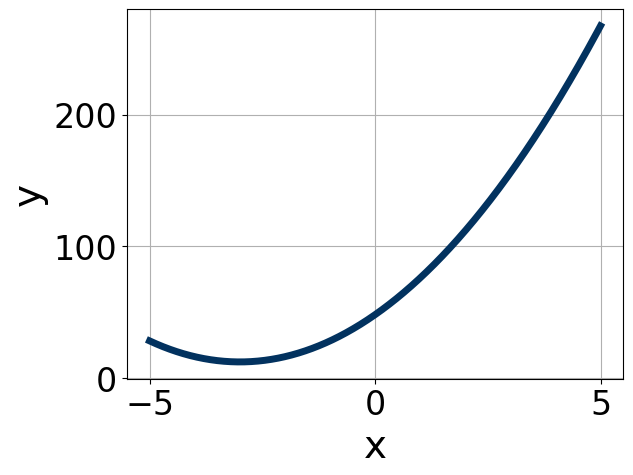
\includegraphics[width = 0.3\textwidth]{../Figures/quadraticEquationToGraphAC.png}\item 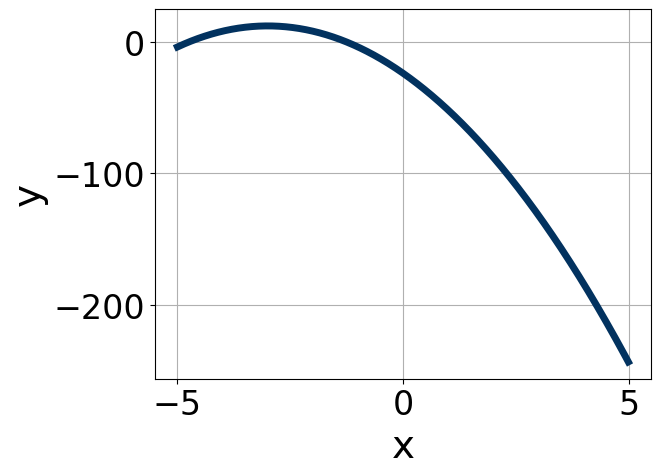
\includegraphics[width = 0.3\textwidth]{../Figures/quadraticEquationToGraphBC.png}\item 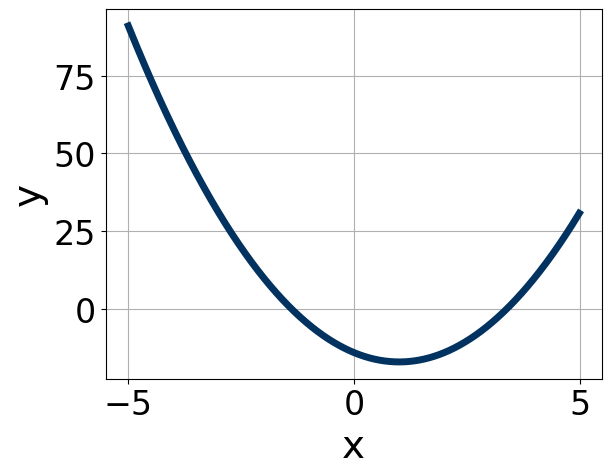
\includegraphics[width = 0.3\textwidth]{../Figures/quadraticEquationToGraphCC.png}\item 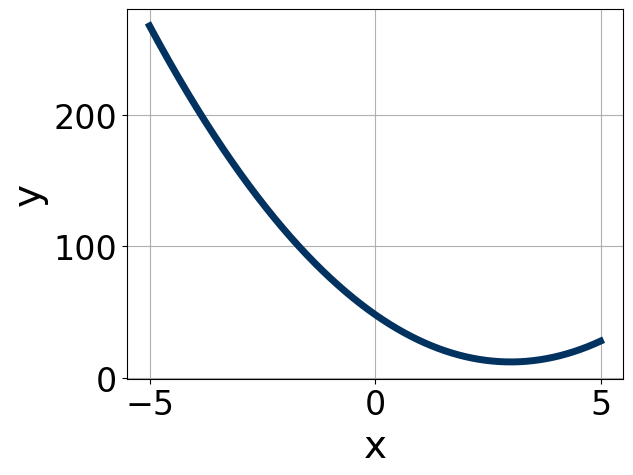
\includegraphics[width = 0.3\textwidth]{../Figures/quadraticEquationToGraphDC.png}\end{multicols}\item None of the above.
\end{enumerate} }
\litem{
Write the equation of the graph presented below in the form $f(x)=ax^2+bx+c$, assuming  $a=1$ or $a=-1$. Then, choose the intervals that $a, b,$ and $c$ belong to.
\begin{center}
    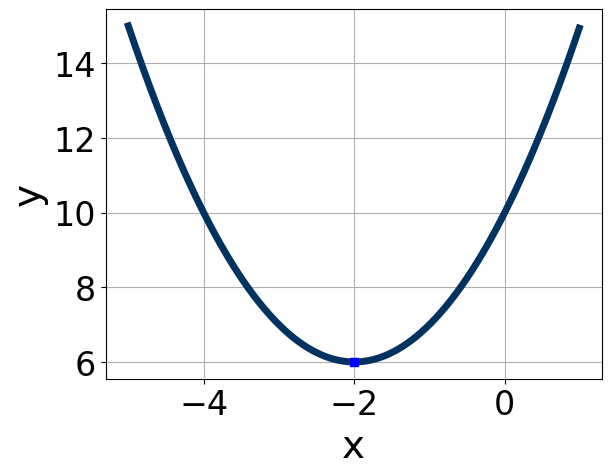
\includegraphics[width=0.5\textwidth]{../Figures/quadraticGraphToEquationCopyC.png}
\end{center}
\begin{enumerate}[label=\Alph*.]
\item \( a \in [0.7, 1.5], \hspace*{5mm} b \in [3, 8], \text{ and } \hspace*{5mm} c \in [8, 11] \)
\item \( a \in [-3.2, -0.3], \hspace*{5mm} b \in [-4, -2], \text{ and } \hspace*{5mm} c \in [2, 3] \)
\item \( a \in [0.7, 1.5], \hspace*{5mm} b \in [-4, -2], \text{ and } \hspace*{5mm} c \in [-2, -1] \)
\item \( a \in [-3.2, -0.3], \hspace*{5mm} b \in [3, 8], \text{ and } \hspace*{5mm} c \in [2, 3] \)
\item \( a \in [0.7, 1.5], \hspace*{5mm} b \in [-4, -2], \text{ and } \hspace*{5mm} c \in [8, 11] \)

\end{enumerate} }
\end{enumerate}

\end{document}